\documentclass[]{article}
\renewcommand{\baselinestretch}{1.25}

\usepackage[margin=1in]{geometry}
\usepackage{physics}
\usepackage{amsmath, amsfonts, amssymb, amsthm}
\usepackage{amssymb}
\usepackage{graphicx}
\usepackage{hyperref}
\usepackage{empheq}

% MATLAB Formatting Code
\usepackage[numbered,framed]{matlab-prettifier}
\lstset{style=Matlab-editor,columns=fullflexible}
\renewcommand{\lstlistingname}{Script}
\newcommand{\scriptname}{\lstlistingname}

% TikZ Things
\usepackage{tikz}
\usetikzlibrary{positioning,shapes}


% Formatting Preferences
\numberwithin{equation}{section}
\usepackage{parskip}
\renewcommand{\figurename}{Fig.}
\allowdisplaybreaks

% Section Heading Settings
\usepackage{enumitem}
\renewcommand{\theenumi}{\alph{enumi}}
\renewcommand*{\thesection}{Problem \arabic{section}}
\renewcommand*{\thesubsection}{\alph{subsection})}
\renewcommand*{\thesubsubsection}{\quad \quad \roman{subsubsection})}

% Math Proof things
\newcommand{\Rel}{\mathcal{R}}
\newcommand{\R}{\mathbb{R}}
\newcommand{\C}{\mathbb{C}}
\newcommand{\N}{\mathbb{N}}
\newcommand{\Z}{\mathbb{Z}}
\newcommand{\Q}{\mathbb{Q}}

\newcommand{\st}{\ : \ }

% Theorem Definition
\newtheorem{definition}{Definition}
\newtheorem{assumption}{Assumption}
\newtheorem{theorem}{Theorem}
\newtheorem{lemma}{Lemma}
\newtheorem{proposition}{Proposition}
\newtheorem{example}{Example}


% Multiagent Robotic Systems Commands
\newcommand{\diam}{\textnormal{diam}}
\newcommand{\radius}{\textnormal{radius}}




%opening
\title{MECH 6V29: Multiagent Robotic Systems- HW 2}
\author{Jonas Wagner}
\date{2022, March 1\textsuperscript{st}}

\begin{document}	

\maketitle

\tableofcontents

%----------------------------------------------------------------------------

% Problem 1 -------------------------------------------------
\newpage
\section{}
% \textbf{Problem:} 
State a summary of lectures \emph{\textbf{lectures 6-10}}, preferably by creating a concept map diagram (flow diagram). 
The whole purpose is to make sure that we are clear about the bigger picture, 
and reiterate why are we doing and discussing the specific topics in the class. 
Do not merely write the topics, instead create connections between topics to clarify the flow of information.

\subsection{Big Picture Chart}
\begin{figure}[h]
	\centering
    \resizebox*{\textwidth}{!}{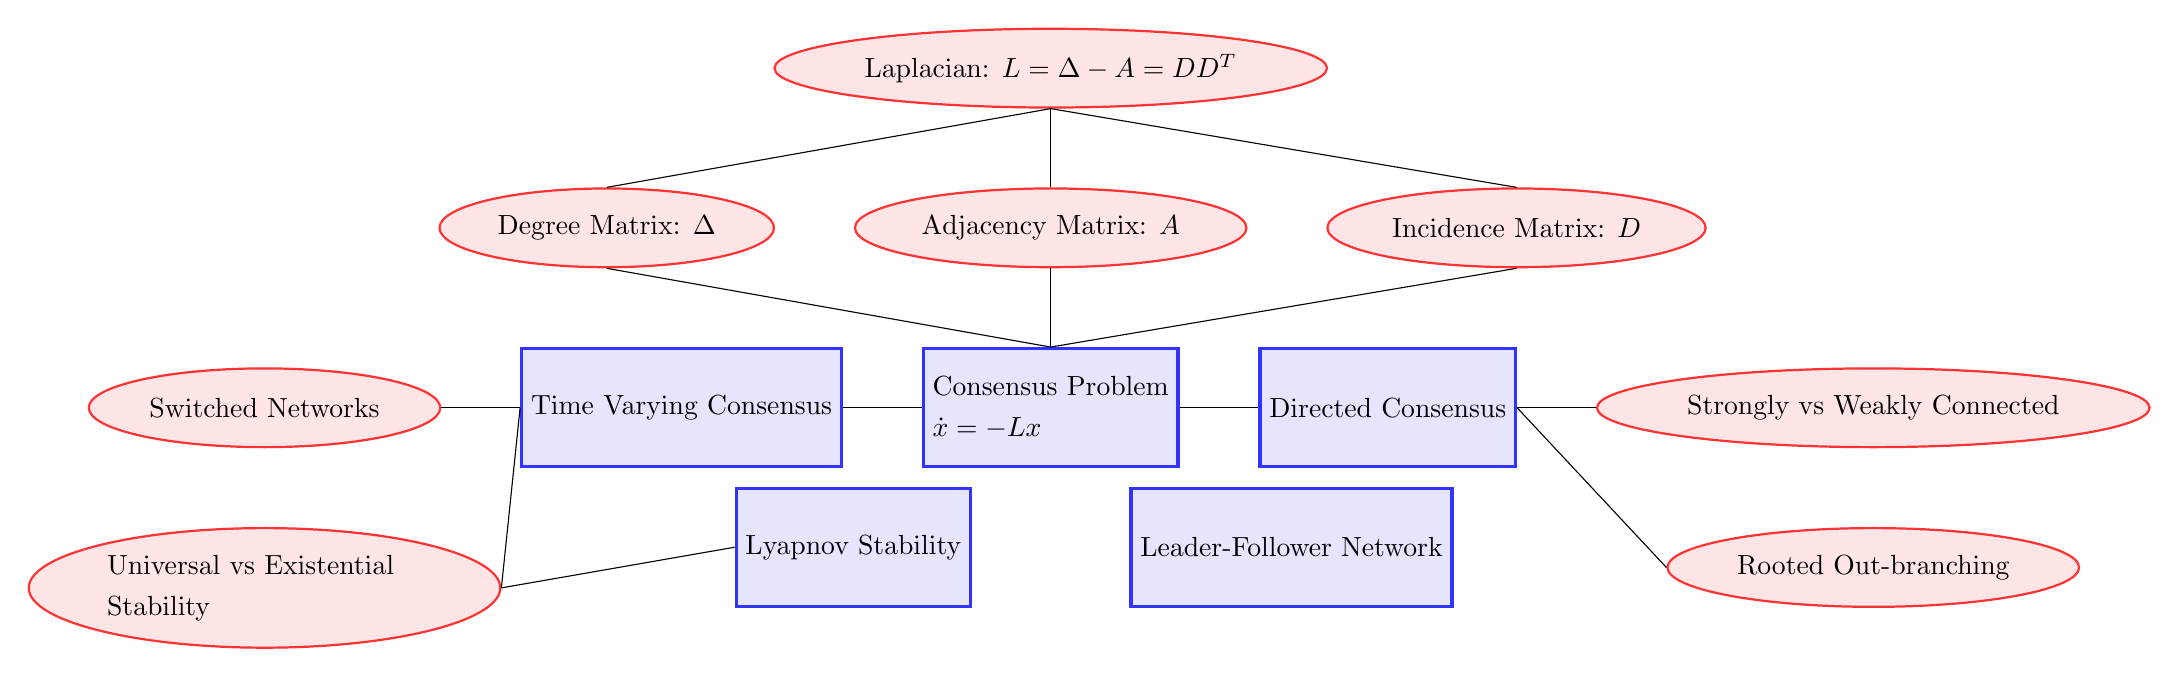
\begin{tikzpicture}[
		empty/.style={coordinate, draw=white!0, fill=white!0, thin, minimum size = 0.1mm},
		block/.style={rectangle, draw=blue!80, fill=blue!10, very thick, minimum size = 15mm},
		extra/.style={ellipse, draw=red!80, fill=red!10, thick, minimum size = 10mm},
		auto,
		% roundnode/.style={circle, draw=green!60, fill=green!5, very thick, minimum size=7mm},
		% squarednode/.style={rectangle, draw=red!60, fill=red!5, very thick, minimum size=5mm},
		]
		%Main Nodes
		\node[empty]	(center)								{};
		\node[block, text width = 30mm]	(consensus)	[above=of center]	{Consensus Problem $\dot{x}=-L x$};
		\node[block]	(lyap)		[left=of center] 	{Lyapnov Stability};
		\node[block]	(lead_follow)		[right=of center] 	{Leader-Follower Network};
        % \node[block]	(applications)		[below=of center]	{Real-world Applications};

        %Consensus
        \node[extra]	(con_2)		[above=of consensus]	{Adjacency Matrix: $A$};
        \node[extra]	(con_1)		[left=of con_2]			{Degree Matrix: $\Delta$};
        \node[extra]	(con_3)		[right=of con_2]		{Incidence Matrix: $D$};
        \node[extra]	(con_4)		[above=of con_2]		{Laplacian: $L = \Delta - A = DD^T$};
        \draw[-]	(consensus.north) 	--	(con_1.south);
        \draw[-]	(consensus.north) 	--	(con_2.south);
        \draw[-]	(consensus.north) 	--	(con_3.south);
        \draw[-]	(con_1.north)		--	(con_4.south);
        \draw[-]	(con_2.north)		--	(con_4.south);
        \draw[-]	(con_3.north)		--	(con_4.south);

        %Directed Consensus
        \node[block]	(di_con)	[right=of consensus]	{Directed Consensus};
        \draw[-]    (consensus.east) -- (di_con.west);
        \node[extra]    (di_con_1)  [right=of di_con]    {Strongly vs Weakly Connected};
        \draw[-]    (di_con.east) -- (di_con_1.west);
        \node[extra]    (di_con_2)  [below=of di_con_1]    {Rooted Out-branching};
        \draw[-]    (di_con.east) -- (di_con_2.west);

        %Time-Varying Consensus
        \node[block]	(tv_con)	[left=of consensus]	{Time Varying Consensus};
        \draw[-]    (consensus.west) -- (tv_con.east);
        \node[extra]    (tv_con_1) [left=of tv_con] {Switched Networks};
        \draw[-]    (tv_con.west) -- (tv_con_1.east);
        \node[extra, text width = 40mm]    (tv_con_2) [below=of tv_con_1] {Universal vs Existential Stability};
        \draw[-]    (tv_con.west) -- (tv_con_2.east);
        \draw[-]    (lyap.west) -- (tv_con_2.east);

        %Leader-Follower System
        % \node[extra] 

		% %Main Lines
		% \draw[-] (applications.west) 	.. controls +(left:5mm) and +(up:3mm)  ..	(ctrl_pblms.north); %controls +(up:5mm) and +(left:5mm)
		% \draw[-] (applications.east) 	.. controls +(right:5mm) and +(up:3mm) .. (network_model.north);
		% \draw[-] (ctrl_pblms.south) 	.. controls +(down:7mm) and +(left:7mm)  .. (consensus.west);
		% \draw[-] (network_model.south)	.. controls +(down:7mm) and +(right:7mm) ..	(consensus.east);

		% %Applications
		% \node[extra]	(app_2)		[below=of applications]	{``Smart'' Grids};
		% \node[extra]	(app_1)		[left=of app_2]			{Groups of UAVs};
		% \node[extra]	(app_3)		[right=of app_2]		{Comm Networks};
		% \draw[-]	(applications.south) -- (app_1.north);
		% \draw[-]	(applications.south) -- (app_2.north);
		% \draw[-]	(applications.south) -- (app_3.north);

		% %Control Problems
		% \node[extra]	(ctr_2)		[left=of ctrl_pblms]	{Formation};
		% \node[extra]	(ctr_1)		[above=of ctr_2]		{Rendezvous};
		% \node[extra]	(ctr_3)		[below=of ctr_2]		{Flocking};
		% \draw[-]	(ctrl_pblms.west)	--	(ctr_1.east);
		% \draw[-]	(ctrl_pblms.west)	--	(ctr_2.east);
		% \draw[-]	(ctrl_pblms.west)	--	(ctr_3.east);

		% %Network Models
		% \node[extra]	(graph_2)	[right=of network_model]	{Dynamic vs Static};
		% \node[extra]	(graph_1)	[above=of graph_2]			{Proximity-Based};
		% \node[extra]	(graph_3)	[below=of graph_2]			{Directed vs Undirected};
		% \draw[-]	(network_model.east)	--	(graph_1.west);
		% \draw[-]	(network_model.east)	--	(graph_2.west);
		% \draw[-]	(network_model.east)	--	(graph_3.west);

		

	\end{tikzpicture}}
	\caption{Diagram of Course Topics (created w/ TikZ)}
	\label{fig:pblm1}
\end{figure}

% Problem 2 -------------------------------------------------
\newpage
\section{}
Recall that if $x_i$ is scalar, with its derivative given by the consensus equation \[
    \dot{x}_i = \sum_{j \in \mathcal{N}_i} (x_j - x_i), \ i = 1, 2, \cdots, N
\] this can be written as \[
    \dot{x} = - L x
\] where $L$ is the Laplacian of the undirected graph, 
and $x = \mqty[x_1 x_2 \cdots x_N]^T$.

\subsection{}
\subsubsection*{Problem:}
If instead\[
    \dot{x} = - L^2 x
\] what are the corresponding node level dynamics, that is, find \[
    \dot{x}_i = ???
\]
\subsubsection*{Preliminaries}
\begin{definition} \label{def:graph_matrices}
	Let graph $G(V,E)$ with $V = \qty{v_1,\dots,v_n}$ and $E \subseteq V \cross V$.
	\begin{enumerate}
		\item The \underline{\emph{degree matrix}} $\Delta \in \R^{n\cross n}$ is a diagonal matrix defined as \[
			\Delta := \mqty[\dmat{\deg(v_1), \deg(v_2), \ddots, \deg(v_n)}]
		\]
		\item The \emph{\underline{adjacency matrix}} $A \in \R^{n\cross n}$ is a symmetric matrix $(A = A^T)$ defined s.t. \[
			A = [a_{ij}] \st a_{ij} \begin{cases}
				1 &(v_i,v_j) \in V\\
				0 &(v_i,v_j) \notin V
			\end{cases}
		\]
		\item The \emph{\underline{incidence matrix}} $D \in \R^{n \cross m}$ is defined as\[
			D = [d_{ij}] \st d_{ij} \begin{cases}
				1 	&(v_i,-) \in e_{j}\\
				-1	&(-,v_i) \in e_{j}\\
				0	&\text{otherwise}
			\end{cases}
		\]
		\item The \emph{\underline{Laplacian matrix}} $L \in \R^{n \cross n}$ is a symmetric $(L = L^T)$ and strictly semi-positive definite $(L \succeq 0)$ is defined as\[
			L := \Delta - A = D D^T
		\]and\[
			L = \mqty[
				\deg(v_1)	&-a_{12}	&-a_{13}	&\cdots	&-a_{1n}\\
				-a_{21}		&\deg(v_2)	&-a_{23}	&\cdots	&-a_{2n}\\
				\vdots		&\vdots		&\vdots		&\ddots	&\vdots\\
				-a_{n1}		&-a_{n2}	&-a_{n3}	&\cdots	&\deg(v_n)
			]
		\]
		\item For a weighted graph $G(V,E,W)$, the diagonal weighted matrix $W\in \R^{m\cross m}$ is defined as\[
			W = [w_{ij}] \forall_{ij \in E}
		\]
		were $w_{ij}$ are the corresponding weights for $e_{ij} = (v_i,v_j)$.
	\end{enumerate}
\end{definition}

\begin{definition} \label{def:consensus_dynamics}
	Let undirected and unweighted graph $G(V,E)$ with $V = \qty{v_1,\dots,v_n}$ and $E \subseteq V \cross V$.
	The \emph{\underline{consensus dynamics}} of network $G(V,E)$ is defined by\[
		\forall_{i=1,\dots,n} \ \dot{x}_i = \sum_{j\in \mathcal{N}_i} (x_j - x_i)
		\iff \dot{x} = -L x
	\] For the case with weighted graph $G(V,E,W)$ with diagonal weight matrix $W = [w_{ij}]$, 
	\emph{\underline{weighted consensus dynamics}} are given as\[
		\dot{x}_i = \sum_{j\in\mathcal{N}_i} w_{ij} (x_j - x_i) 
		\implies \dot{x} = - L_{w} x
	\]where weighted Laplacian matrix $L_{w}$ is defined as\[
		L_{w} = D W D^T
	\]
\end{definition}


\subsubsection*{Solution:}
From the definition of the Laplacian Matrix (Definition \ref{def:graph_matrices}), we have\[
    L = \Delta - A
\] and therefore \begin{align*}
    L^2 &= L * L = (\Delta - A) (\Delta - A)\\
        &= \Delta^2 - \Delta A - A \Delta + A^2\\
        &= \mqty[
            \deg(v_1)^2	&0	&0	&\cdots	&0\\
            0		&\deg(v_2)^2	&0	&\cdots	&0\\
            \vdots		&\vdots		&\vdots		&\ddots	&\vdots\\
            0		&0	&0	&\cdots	&\deg(v_n)^2
        ] \\ &\qquad + \mqty[
            0	&-a_{12} \deg(v_1)	&-a_{13} \deg(v_1)	&\cdots	&-a_{1n} \deg(v_1)\\
            -a_{21}	\deg(v_2)	&0	&-a_{23} \deg(v_2)	&\cdots	&-a_{2n} \deg(v_2)\\
            \vdots		&\vdots		&\vdots		&\ddots	&\vdots\\
            -a_{n1}	\deg(v_n)	&-a_{n2} \deg(v_n)	&-a_{n3} \deg(v_n)	&\cdots	&0
        ] \\ &\qquad + \mqty[
            0	&-a_{12} \deg(v_1)	&-a_{13} \deg(v_2)	&\cdots	&-a_{1n} \deg(v_3)\\
            -a_{21}	\deg(v_1)	&0	&-a_{23} \deg(v_2)	&\cdots	&-a_{2n} \deg(v_3)\\
            \vdots		&\vdots		&\vdots		&\ddots	&\vdots\\
            -a_{n1}	\deg(v_1)	&-a_{n2} \deg(v_2)	&-a_{n3} \deg(v_3)	&\cdots	&0
        ] \\ &\qquad + \mqty[
            \sum_{i \neq 1}^n a_{1,i} a_{i,1} & \sum_{i \neq 1,2} a_{1,i} a_{i,2} & \cdots &\sum_{i \neq 1,n} a_{1,i} a_{i,2}\\
            \sum_{i \neq 2,1} a_{2,i} a_{i,1} & \sum_{i \neq 2} a_{2,i} a_{i,2} & \cdots & \sum_{i \neq 1,n} a_{1,i} a_{i,n}\\
            \vdots  &  \vdots &\ddots &\vdots\\
            \sum_{i \neq n,1} a_{n,i} a_{i,1} & \sum_{i \neq n,2} a_{n,i} a_{i,2} &\cdots &\sum_{i\neq n} a_{n,i} a_{i,n}
        ]
\end{align*}
which results in \[\boxed{
    \dot{x}^{(i)} = - \qty(\deg(v_1)^2 + \sum_{j \neq i} a_{i,j} a_{j,i}) x^{(i)} 
                    - \sum_{j \neq i} \qty(-a_{i,j} (\deg(v_i) + \deg(v_j)) + \sum_{k \neq j} a_{i,k} a_{k,j}) x^{(j)}
}\]

\subsection{}
\subsubsection*{Problem:}
Can you give a graph-theoretic interpretation to your answer in $(A)$?

\subsubsection*{Solution:}
A potential graph-theoretical interpretation could be would be a 










% Problem 3 -------------------------------------------------
\newpage
\section{}
Consider a leader-follower network with two leaders and two followers, as shown in \figurename \ref{fig:pblm3}. 
Assume that leaders and followers are on the real line, and the underlying network graph is a path graph with the end nodes being the static leaders.
Moreover, let the dynamics be given by the following:
\begin{gather*}
    \dot{x}_1 = \alpha_1((x_3-x_1) + (x_2 - x_1))\\
    \dot{x}_2 = \alpha_2((x_1-x_2) + (x_4 - x_2))\\
    \dot{x}_3 = \dot{x}_4 = 0
\end{gather*}
Where to $x_1$ and $x_2$ end up as $t \to \infty$ if $x_3 = \beta$ and $x_4 = \gamma$?

\begin{figure}[h]
    \centering
    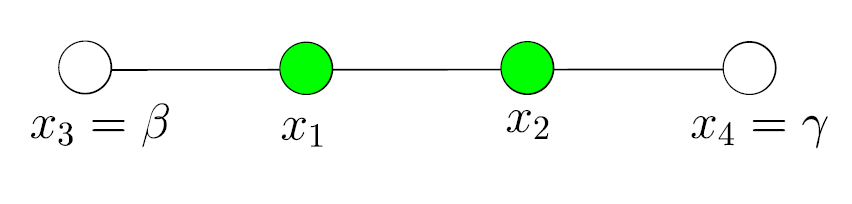
\includegraphics[width=0.7\textwidth]{figs/pblm3.png}
    \caption{Leader-follower Network}
    \label{fig:pblm3}
\end{figure}

\subsection*{Solution:}
The dynamics of the network overall are described by the dynamics $\dot{x} = A_cls x$ with matrix \[
    A_{cls} = \mqty[
        -2 \alpha_1 & \alpha_1 & \alpha_1 &0\\
        \alpha_2 & - 2 \alpha_2 & 0 & \alpha_2\\
        0  & 0 & 0 & 0\\
        0  & 0 & 0 & 0
    ]
\] This can further be redefined into the dynamical system $\dot{x} = A x + B u$ with matrices \[
    A = \mqty[
        -2 \alpha_1 & \alpha_1\\
        \alpha_2    & -2 \alpha_2
    ]
\] \[
    B = \mqty[\dmat{
        \alpha_1,
        \alpha_2
    }]
\] where $u$ is the static "input" of \[
    u = \mqty[
        \beta\\
        \gamma
    ]
\]

Assuming that $\alpha_1, \alpha_2 > 0$, $A$ is stable and therefore the system wll decay to the reference signal $u$.
\emph{Note:} If $u$ changes then the response would be governed by transfer function $(s I - A)^{-1} B$.
The final state will be the solution to \[
    \dot{x} = 0 = A_{cls} x = A x + B u
\] which is calculated to be \[\boxed{
    x_{\infty} = \mqty[
        \cfrac{2 \beta + \gamma}{3}\\
        \cfrac{\beta + 2 \gamma}{3}
    ]
}\]
    

% Problem 4 -------------------------------------------------
\newpage
\section{}
\subsection*{Problem:}
Given an undirected network containing a total of $N$ nodes. 
There is a single anchor node that is connected to every one of the follower nodes, that is, anchor has a degree of $N-1$. 
Find the simple expression for the following quantities.
\begin{enumerate}
    \item $l$
    \item $L_f \vb{1}$
\end{enumerate}
where $L_f$ is the matrix obtained from the partition of the Laplacian matrix as we discussed in class.

Also, relate your answers to where the followers end up as $t \to \infty$.

\subsection*{Preliminaries:}
\begin{definition}\label{def:leader_follower_dynamics}
    Let undirected and unweighted graph $G(V,E)$ with $V = \qty{v_1,\dots,v_n}$ and $E \subseteq V \cross V$.
    Vertices in $V$ are classified as either \emph{leaders} ($v_i \in V_l$) or \emph{followers} ($v_i \in V_f)$. 
	The \emph{\underline{leader-follower}} dynamics of the states within network $G(V,E)$ are defined by\[\begin{cases}
        \dot{x}_i = - \sum_{j \neq N_i} (x_i - x_j) &\forall_{i \st v_i \in V_{f}}\\
        \dot{x}_i =  0 &\forall_{i \st v_i \in V_{l}}
    \end{cases}
	\] or equivalently when $V_{l} = \{v_n\}$ (single leader node) \[
        \dot{x} = \mqty[
            -L_f & - l\\
            0 & 0
        ]
    \]
\end{definition}

\subsection*{Solution:}
Assuming that the network is unweighted and the single leader is associated with $v_n$,\[
    \dot{x} = \mqty[
        -L_f & - l\\
        0 & 0
    ]
\]
\subsubsection{$l$}
Since $\deg(v_n) = N-1$, \[
    \sum_{i=1}^{N-1} l_i = N-1
\] therefore all elements must be 1 and \[
    l = \mathbf{1}_{N-1}
\]

\subsubsection{$L_f \mathbf{1}$}

\begin{align*}
    L_f \mathbf{1} 
        &= \mqty[
            \deg(v_1) & -a_{1,2} &\cdots &-a_{1,n}\\
            -a_{2,1} &\deg(v_2)  &\cdots &-a_{2,n}\\
            \vdots &\vdots &\ddots &\vdots\\
            -a_{n,1} &-a_{n,2} &\cdots &\deg(v_n)
        ] \mqty[
            1\\
            1\\
            \vdots\\
            1  
        ]
        &= \mqty[
            \deg(v_1) - \sum_{i \neq 1} a_{1,i}\\
            \deg(v_2) - \sum_{i \neq 2} a_{2,i}\\
            \vdots\\
            \deg(v_n) - \sum_{i \neq n} a_{n,i}\\
        ]
    \intertext{Since by definition $\deg(v_i) = \sum{j\neq i} a_{i,j}$,}
    \Aboxed{
    L_f \mathbf{1} 
        &= \mqty[
            0\\
            0\\
            \vdots\\
            0
        ] = \mathbf{0}_{N-1}}
\end{align*}



% Problem 5 -------------------------------------------------
\newpage
\section{}
\subsection*{Problem:}
Consider the (undirected) network in \figurename \ref{fig:pblm5}. 
At any instance of time, exactly one of the nodes $x$ and $y$ would be included in the network. 
So, basically, we will get a switched system. 
Assuming all nodes impliment the consensus dynamics, will they converge at one point (centroid of initial states) asymptotically?
Explain.
\begin{figure}[h]
    \centering
    % 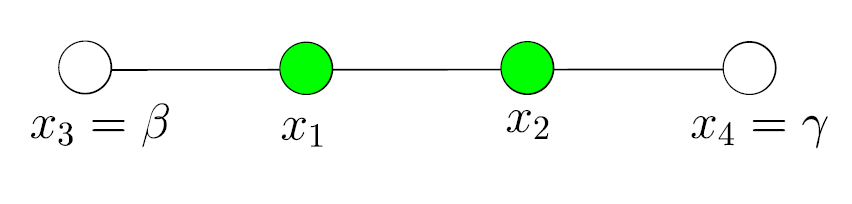
\includegraphics[width=0.3\textwidth]{figs/pblm3.png}
    \caption{Network for problem 5}
    \label{fig:pblm5}
\end{figure}

\subsection*{Preliminaries:}
Include Theorems related to requirements to switched system stability... 

\subsection*{Solution:}
Within this switched system shown in \figurename \ref{fig:pblm5}, the exclusion of nodes $x$ and $y$ during any singe time-step causes the system to be disconnectd into 2 connected subgraphs. 








% $K_{1,6}$ is a star graph with one central node and six leaf nodes as shown in \figurename\ref{fig:pblm5}

% \begin{figure}[h]
% 	\centering
% 	% 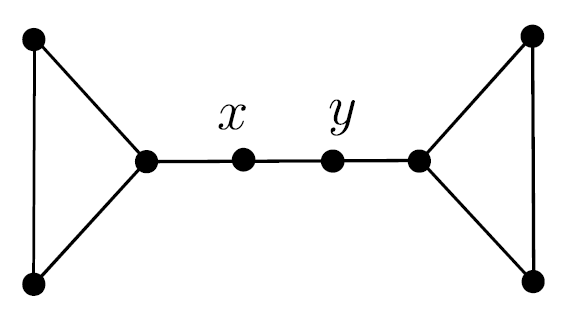
\includegraphics[width=0.2\textwidth]{figs/pblm5.png}
% 	\caption{Star graph, $K_{1,6}$.}
% 	\label{fig:pblm5}
% \end{figure}

% Your task is to show that $K_{1,6}$ can never be an induced subgraph of a $\Delta$-disk proximity graph.

% \subsection{Definitions:}
% \begin{definition}\label{def:induced_subgraph}
% 	Let $G(V,E)$ with $V = \qty{v_1,v_2,\dots,v_n}$ 
% 	and $E = \qty{e_1, \dots, e_m} \subseteq V \cross V$ 
% 	with $e_k = e_{ij} = (v_i, v_j)$.
% 	An \emph{\underline{induced subgraph}} of $G(V,E)$ is any $G(V',E')$ with $V'\subset V$ and $E' = [e_{ij}] \ \forall_{v_i, v_j \in V'}$
% \end{definition}

% \begin{definition}\label{def:Delta-disk_graph}
% 	Let $V = \qty{v_1,v_2,\dots,v_n}$ be vertices.
% 	\emph{\underline{$\Delta$-Disk Graphs}} are constructed for a particular $\Delta$ such that \[
% 		(v_i,v_j) \in E \iff \norm{v_i,v_j} \leq \Delta
% 	\]
% \end{definition}

% \subsection{Solution:}
% \begin{theorem}
% 	Let $G(V,E)$ be a $\Delta$-Disk Graph for an arbitrary $\Delta$.
% 	The star graph $K_{1,6} = G(V_{k16},E_{k16})$ can never be an induced sub graph of $G(V,E)$.
% 	\begin{proof}
% 		By Definition \ref{def:Delta-disk_graph}, \[
% 			E = [e_{ij}] \st e_{ij} = (v_i,v_j) \iff \norm{v_i,v_j} \leq \Delta
% 		\] Similarly, by Definition \ref{def:induced_subgraph}, an induced subgraph of $G(V,E)$ for vertex set $V' \subset V$ is defined by $G(V',E')$ where $E' = [e_{ij}] \ \forall_{v_i, v_j \in V'}$.
% 		The associated induced subgraph of $G(V,E)$ for $V' = V_{k16}$ has edges $E' = [e_{ij}] \ st e_{ij} = (v_i,v_j) \iff \norm{v_i,v_j} \leq \Delta$.
% 		It is clear that for the vertices in $K_{1,6}$, the edges included in $E_{k16}$ is a strict subset of of those within an induced subgraph of those same vertices.
% 		More simplistically, the edges connecting neighboring leaf nodes that satisfy $\norm{v_i,v_j} \leq \Delta$ would be required for it to be an induced subgraph of a $\Delta$-Disk graph.
% 	\end{proof}
% \end{theorem}

% Problem 6 -------------------------------------------------
\newpage
\section{}
% If $l_{i,j}$ is the shortest path distance (number of edges one needs to follow) between vertices $v_i$ and $v_j$, 
% the diameter of the graph is defined as\[
% 	\diam(G) = \max_{v_i,v_j \in V} l_{i,j}
% \] Similarly, if we let $l_{i}^{*}$ (known as the eccentricity of vertex $v_i$) be the longest distance to any vertex from the vertex $v_i$, i.e.,\[
% 	l_{i}^{*} = \max_{v_j \in V} l_{i,j}
% \] then the radius of a graph is defined as\[
% 	\radius(G) = \min_{v_i \in V} l_{i}^{*}
% \] Find the radius and diameter of the following graphs.

% \begin{figure}[h]
% 	\centering
% 	% 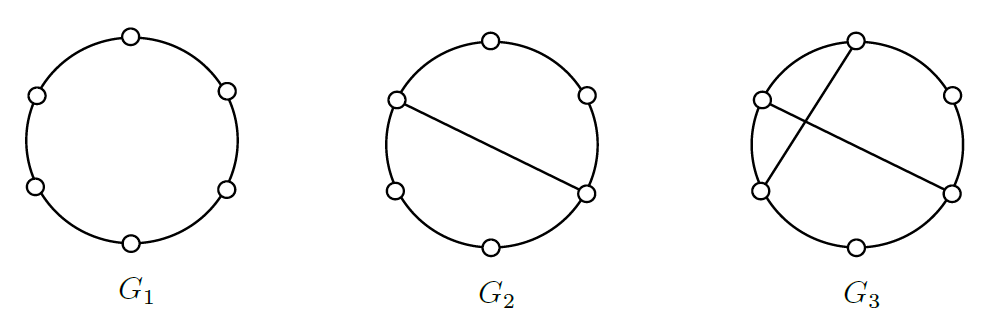
\includegraphics[width=0.7\textwidth]{figs/pblm6.png}
% 	\caption{Graphs $G_1$, $G_2$, and $G_3$.}
% 	\label{fig:pblm6}
% \end{figure}

% \subsection{Definitions:}
% \begin{definition}\label{def:path_diam_radius_etc}
% 	Let $G(V,E)$ be a undirected graph with $V = \qty{v_1,v_2,\dots,v_n}$ 
% 	and $E = \qty{e_1, \dots, e_m} \subseteq V \cross V$ 
% 	with $e_k = e_{ij} = (v_i, v_j)$.
% 	\begin{enumerate}
% 		\item A \emph{\underline{path}} between two vertices $v_i$ and $v_j$ is a sequence of edges $[e_{i, *}, \dots, e_{*, j}]$ that joins a sequence of vertices $[v_i, \dots, v_j]$.
% 		\item A \emph{\underline{path length}} is the number of edges in the path. 
% 		\item The \emph{\underline{shortest path length}} $l_{i,j}$ is the minimum length of all paths between vertices $v_i$ and $v_j$. 
% 		This quantity is also known as the \emph{\underline{distance}} between $v_i$ and $v_j$, $\text{dist}\qty(v_i,v_j)$.
% 		\item The \emph{\underline{diameter}} of graph $G(V,E)$ is the maximum distance between any two vertices in the graph. 
% 		(i.e.)\[
% 			\diam(G(V,E)) := \max_{v_i,v_j \in V} l_{i,j}
% 		\]
% 		\item The \emph{\underline{eccentricity}} of vertex $v_i$, $l_{i}^{*}$, is the largest distance from $v_i$ to any other vertex in the graph. 
% 		(i.e)\[
% 			l_{i}^{*} := \max_{v_j \in V} l_{i,j}
% 		\]
% 		\item The \emph{\underline{radius}} of graph $G(V,E)$ is the minimum eccentricity of the vertices of the graph.
% 		(i.e)\[
% 			\radius(G(V,E)) := \min_{v_i \in V} l_{i}^{*} = \min_{v_i \in V} \max_{v_j \in V} l_{i,j}
% 		\]
% 	\end{enumerate}
% \end{definition}

% \subsection{Solution}
% \begin{enumerate}
% 	\item $G_1$
% 	\begin{enumerate}
% 		\item $\diam(G_1) = 3$
% 		\item $\radius(G_1) = 3$
% 	\end{enumerate}
% 	\item $G_2$
% 	\begin{enumerate}
% 		\item $\diam(G_2) = 4$
% 		\item $\radius(G_2) = 2$
% 	\end{enumerate}
% 	\item $G_3$
% 	\begin{enumerate}
% 		\item $\diam(G_3) = 2$
% 		\item $\radius(G_3) = 2$
% 	\end{enumerate}
% \end{enumerate}

% Problem 7 -------------------------------------------------
\newpage
\section{}
% Following are some undirected networks on four nodes with the same initial positions.
% In which of these networks, nodes converge fastest under the distributed consensus dynamics? 
% Explain your answer.

% \begin{figure}[h]
% 	\centering
% 	% 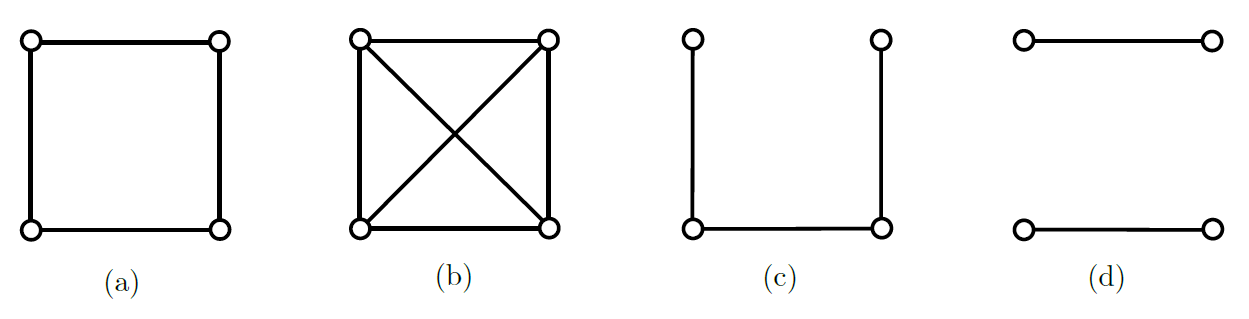
\includegraphics[width=0.7\textwidth]{figs/pblm7.png}
% 	\caption{Four node undirected networks}
% 	\label{fig:pblm7}
% \end{figure}

% \subsection{Network Modeling}
% Let vertices $V = \qty{v_1, v_2, v_3, v_4}$ represent each of the 4 nodes in the undirected networks shown in \figurename \ \ref{fig:pblm7}.
% Take vertices $v_1, v_2, v_3,$ and $v_4$ as top-left, top-right, bottom-left, and bottom-right respectively.

% The edge sets for each network, $\qty{E_a, E_b, E_c, E_d}$, are as follows:
% \begin{enumerate}
% 	\item $E_a = \qty{(v_1,v_2), (v_1, v_3), (v_2,v_4), (v_3,v_4)}$
% 	\item $E_b = \qty{(v_1,v_2), (v_1, v_3), (v_1,v_4), (v_2,v_3), (v_2,v_4), (v_3,v_4)}$
% 	\item $E_c = \qty{(v_1, v_3), (v_2,v_4), (v_3,v_4)}$
% 	\item $E_d = \qty{(v_1,v_2), (v_3,v_4)}$
% \end{enumerate}

% The Degree $\Delta$, Adjacency $A$, and Laplacian $L$ matrices for each network are laid out in \tablename \ref{tbl:pblm7_matrices}
% \begin{table}
% 	\caption{Network Matrix Representations}
% 	\[\begin{array}{|c|c|c|c|}
% 		\hline
% 			&\Delta &A &L\\
% 		\hline&&&\\
% 		G_a	
% 			&\mqty[\dmat{2,2,2,2}]	
% 			&\mqty[
% 				0	&1	&1	&0\\
% 				1	&0	&0	&1\\
% 				1	&0	&0	&1\\
% 				0	&1	&1	&0
% 			]
% 			&\mqty[
% 				2	&-1	&-1	&0\\
% 				-1	&2	&0	&-1\\
% 				-1	&0	&2	&-1\\
% 				0	&-1	&-1	&2
% 			]\\
% 		&&&\\\hline&&&\\
% 		G_b	
% 			&\mqty[\dmat{3,3,3,3}]	
% 			&\mqty[
% 				0	&1	&1	&1\\
% 				1	&0	&1	&1\\
% 				1	&1	&0	&1\\
% 				1	&1	&1	&0
% 			]
% 			&\mqty[
% 				3	&-1	&-1	&-1\\
% 				-1	&3	&-1	&-1\\
% 				-1	&-1	&3	&-1\\
% 				-1	&-1	&-1	&3
% 			]\\
% 		&&&\\\hline&&&\\
% 		G_c
% 			&\mqty[\dmat{1,1,2,2}]
% 			&\mqty[
% 				0	&0	&1	&0\\
% 				0	&0	&0	&1\\
% 				1	&0	&0	&1\\
% 				0	&1	&1	&0
% 			]
% 			&\mqty[
% 				1	&0	&-1	&0\\
% 				0	&1	&0	&-1\\
% 				-1	&0	&2	&-1\\
% 				0	&-1	&-1	&2
% 			]\\
% 		&&&\\\hline&&&\\	
% 		G_d
% 			&\mqty[\dmat{1,1,1,1}]
% 			&\mqty[
% 				0	&1	&0	&0\\
% 				1	&0	&0	&0\\
% 				0	&0	&0	&1\\
% 				0	&0	&1	&0
% 			]
% 			&\mqty[
% 				1	&-1	&0	&0\\
% 				-1	&1	&0	&0\\
% 				0	&0	&1	&-1\\
% 				0	&0	&-1	&1
% 			]\\
% 		&&&\\\hline
% 	\end{array}\]
% 	\label{tbl:pblm7_matrices}
% \end{table}

% \subsection{Consensus Dynamics}
% From the unweighted consensus dynamics definition in Definition \ref{def:consensus_dynamics}, we have that the continuous time consensus dynamics are governed by the negative Laplacian matrix, $\dot{x} = - L x$.
% The eigenvalues of $L$, \[
% 	\Lambda(L) = \qty{\lambda_1, \lambda_2, \lambda_3, \lambda_4} 
% 	\st 0 = \lambda_1 \leq \lambda_2 \leq \lambda_3, \leq \lambda_4
% \] tell us a lot about the consensus dynamics.
% It is known, from Theorem \ \ref{thm:L_eig_1_eq_zero}, that $\lambda_1 = 0$ and this confirms that $\dim(\textnormal{null}\qty(L)) \geq 1$ and that a stead-state consensus is possible.
% Further, $\lambda_2$ provides us with a lot of information about how quickly the network will (or will not) converge to a single point.
% If $\lambda_2 = 0$, this indicates that the network in not connected and therefore will not converge to a single point due to consensus.
% For $\lambda_2 > 0$, the response associated with the slowest mode will converge along the associated eigenvector direction decaying at $e^{-\lambda_2 t}$; 
% therefore, as $\lambda_2$ increases the faster the network converges.
% Further, this mode will converge to within 2\% of the final location at $t = 4 \lambda_t$.

% \newpage
% \subsection{Solution}
% \textbf{Simple answer:} 
% (b) converges fastest, followed by (a), then (c), while (d) converges to two different locations.

% \textbf{Justified answer:} 
% $\lambda_2$ for each of the networks was calculated as:
% \begin{enumerate}
% 	\item $\lambda_{2}^{(a)} = 2$
% 	\item $\lambda_{2}^{(b)} = 4$
% 	\item $\lambda_{2}^{(c)} = 0.585$
% 	\item $\lambda_{2}^{(d)} = 0$
% \end{enumerate}
% Clearly, \[
% 	\lambda_{2}^{(d)} = 0 < \lambda_{2}^{(c)} < \lambda{2}^{(a)} < \lambda_{2}^{(b)}
% \] 
% $\lambda_{2}^{(d)} = 0$ demonstrates that network (d) is not connected and therefore does not converge.
% Additionally, this demonstrates that the fastest to slowest convergence is (b), (a), then (c).

% Problem 8 -------------------------------------------------
% \newpage
\section{}
% What is the necessary and sufficient condition for the consensus to happen in the case of static directed networks? 
% Derive this condition.

% \subsection{Solution}
% This question isn't very specific about what types of conditions are being referred to, so one of the many equivalent conditions that are both necessary and sufficient is that the the positive semi-definite, yet not generally symmetric, directed Laplacian matrix \[
% 	L = \Delta^{in} - A^{in}
% \] that describes the dynamics of the directed network in consensus as\[
% 	\dot{x} = - L x
% \]\textbf{ has only one zero-valued eigenvalue, $\lambda_1 = 0$, that is associated with eigenvector $\mathbf{1}$}.
% This also is equivalent to saying that the null-space of $L$ is strictly defined as:\[
% 	\textnormal{null}\qty(L) = \textnormal{span}\qty{\mathbf{1}}
% \] The proof of these conditions is simple:

% Consensus occurs when\[
% 	\lim_{t \to \infty} x = x_f \st x_f \in \textnormal{span}\qty{\mathbf{1}}
% \] which is equivalent to saying \[
% 	\textnormal{null}\qty(L) = \textnormal{span}\qty{\mathbf{1}} 
% 	\land L \succeq 0
% \]

% As a linear system $\dot{x} = -L x$ only requires the given $L \succeq 0$ to be considered marginally stable; however explicitly specifying that the associated eigenvector with $\lambda_1 = 0$ is $\mathbf{1}$ is also necessary to ensure that all final states are equivalent.

\newpage
\appendix
\section{MATLAB Code:}\label{apx:matlab}
All code I write in this course can be found on my GitHub repository:\\
\href{https://github.com/jonaswagner2826/MECH6V29_MultiagentRoboticSystems}{https://github.com/jonaswagner2826/MECH6V29\_MultiagentRoboticSystems}

\bibliographystyle{ieeetran}
% \bibliography{refs.bib}
\cite{*}

\end{document}
